\documentclass{book}
\usepackage{graphicx}
\usepackage{enumitem}
\usepackage{../Estilo/modernrules}

\title{Manual do Jogador - ANVESN RPG}
\author{Agência Nacional de Vigilância de Eventos Sobrenaturais}
\date{}

\begin{document}

\maketitle
\begin{center}
\newpage
\vspace*{\fill}
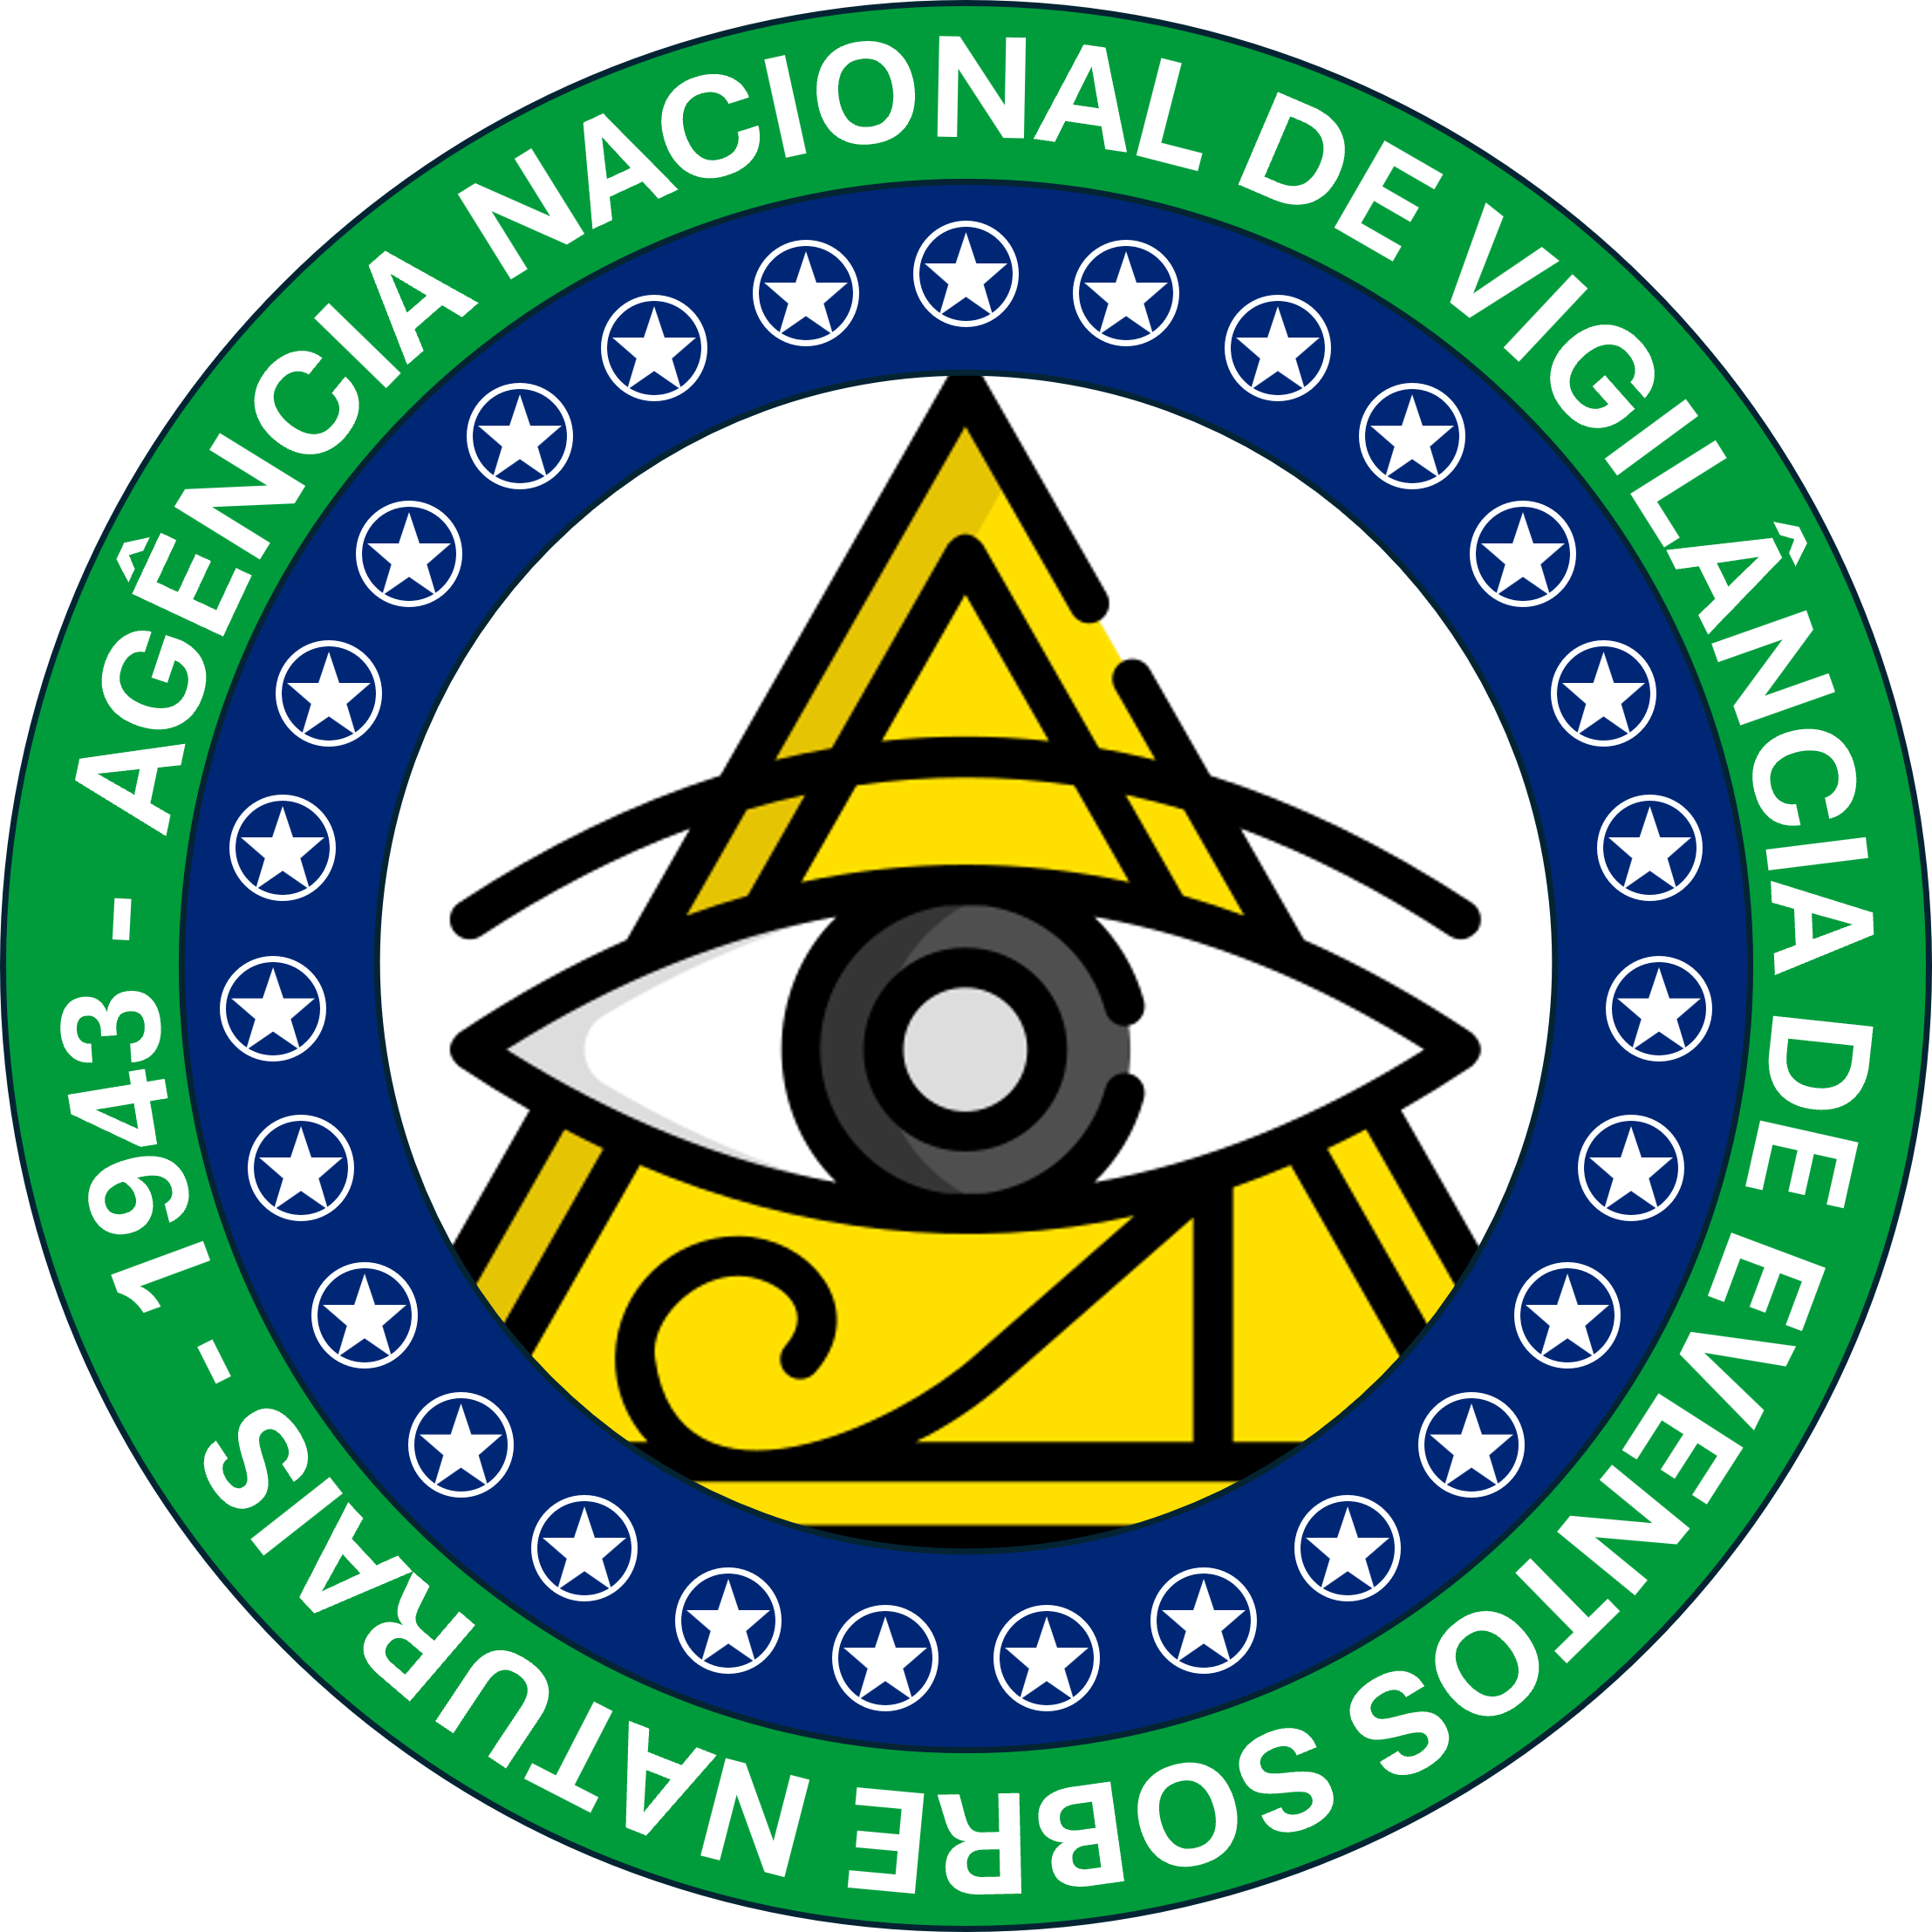
\includegraphics[scale=.9]{imagens/ANVESN_LOGO.png}
\vspace*{\fill}
\newpage
\end{center}

\tableofcontents
\pagestyle{fancy}
% Preâmbulo
\chapter*{Preâmbulo}
Bem-vindo ao Manual do Jogador do ANVESN RPG! Este manual é uma introdução prática para aqueles que desejam se aventurar no mundo das missões da ANVESN, enfrentando entidades e mistérios sobrenaturais. Além das regras e equipamentos, ele também explora histórias de bastidores, fofocas e uma visão mais profunda dos personagens que moldam a agência.

\chapter{Introdução ao Jogo}
\section{O Papel dos Jogadores}
Como jogador, você assume o papel de um agente da ANVESN, um especialista em contenção, análise e combate a ameaças paranormais. Sua missão é preservar a segurança pública enquanto mantém sigilo absoluto sobre as atividades da agência.

\section{Referências às Regras}
Para os detalhes técnicos e mecânicos, consulte o \textbf{Manual de Regras}. Este manual do jogador se concentra nas estratégias de interpretação, uso de equipamentos e adaptação a situações imprevisíveis.

\section{Dicas Práticas de Interpretação e Jogo}
\begin{itemize}
    \item \textbf{Interprete o Passado do Seu Personagem}: Quem é seu personagem? Ele é veterano em investigações paranormais ou um novato destemido? Talvez um ex-policial que foi recrutado após um caso estranho?
    \item \textbf{Crie Laços e Rivalidades}: Os agentes da ANVESN são uma verdadeira família, com todas as tensões que isso implica. Fofocas de bastidores e conflitos pessoais tornam o jogo mais interessante e ajudam a aprofundar os personagens.
    \item \textbf{Priorize o Sigilo e a Segurança}: Missões da ANVESN devem ser discretas. O público não pode descobrir a existência das entidades, então você precisa equilibrar contenção e disfarce.
\end{itemize}

\chapter{Fofocas e Bastidores}
A ANVESN é um ambiente de alta pressão, onde agentes convivem com o sobrenatural diariamente. Entre missões arriscadas e situações inexplicáveis, as fofocas sobre os colegas de trabalho se espalham como fogo. Abaixo estão algumas das histórias mais populares que circulam nos corredores da agência.

\section{Segredos e Conspirações}
\begin{itemize}
    \item Dizem que o Diretor Júlio Antunes, da Diretoria de Poderes Humanos e Super-Humanos, possui poderes místicos próprios. Em uma missão em 2019, ele teria acalmado um poltergeist apenas com sua presença. Os veteranos afirmam que ele era aprendiz de um famoso curandeiro antes de ingressar na ANVESN.
    \item Existe um rumor de que a Diretoria de Alienígenas mantém em sigilo um “Contato”, alguém que já se comunicou com seres extraterrestres. A identidade dessa pessoa é desconhecida, mas há quem diga que a própria agente Camila Ferreira faz visitas noturnas a um laboratório secreto onde o “Contato” é mantido em quarentena.
\end{itemize}

\section{Histórias Sobrenaturais}
\begin{itemize}
    \item Após uma missão, alguns agentes relataram ter visto uma figura estranha andando pelos corredores da sede da ANVESN à noite. Chamam-no de “O Vigilante” e dizem que ele é um espírito que protege a agência. Porém, há quem acredite que seja o espírito de um ex-agente que morreu em serviço e ainda "patrulha" as instalações.
    \item O Dr. Ricardo Siqueira, chefe de pesquisa, nunca dorme dentro das instalações da ANVESN. Alguns dizem que ele sofre de insônia crônica causada por uma exposição a um artefato amaldiçoado, enquanto outros acham que ele está em um pacto com entidades de outro plano e evita dormir para não “ser visitado” por essas entidades.
\end{itemize}

\section{Conflitos e Rivalidades}
\begin{itemize}
    \item Os agentes André Neves e Júlio Antunes raramente concordam. Neves, que comanda a Secretaria de Operações, prefere métodos diretos e físicos, enquanto Antunes acredita no uso de contenção mística e psicológica. Dizem que durante uma missão conjunta, os dois tiveram uma discussão tão intensa que a entidade que estavam enfrentando acabou escapando — e foi vista dias depois em outra cidade.
    \item Há uma rixa antiga entre os agentes que pertencem à Diretoria de Assombrações e Entidades Espirituais e os da Diretoria de Mortos-Vivos. Segundo alguns, a primeira diretoria considera a outra uma “divisão menor”, lidando apenas com “problemas materiais”. Em resposta, a Diretoria de Mortos-Vivos ocasionalmente espalha histórias sobre como espíritos não são nada comparados a um vampiro de verdade.
\end{itemize}

\section{Objetos Curiosos e Relíquias}
\begin{itemize}
    \item Existe um objeto conhecido como “O Amuleto da Morte” que foi guardado na ANVESN há décadas. Ele supostamente dá azar a qualquer um que o toca. Um estagiário recente teria segurado o amuleto por acidente, e desde então, ele sofre de uma série de pequenos infortúnios, como quedas e perda de objetos.
    \item No arsenal da ANVESN, há uma estaca de prata que dizem ter sido usada por um agente veterano em um vampiro. Embora as evidências sejam escassas, a história é contada com orgulho por veteranos, que afirmam que a estaca possui propriedades especiais e deve ser usada apenas em casos extremos.
\end{itemize}

\section{Rituais e Crenças Internas}
\begin{itemize}
    \item Alguns agentes veteranos acreditam que tocar um crucifixo antes de sair para uma missão aumenta as chances de voltar com vida. Dizem que o crucifixo no hall de entrada foi benzido por um padre que também é um exorcista da agência e que ele tem o poder de afastar entidades. O próprio Diretor Antunes teria sido visto tocando o crucifixo discretamente.
    \item Os agentes da Diretoria de Assombrações e Entidades Espirituais têm o costume de carregar um pedaço de sal grosso em seus bolsos, dizendo que ele “corta o caminho” de qualquer espírito hostil. Alguns novatos relatam que, se esquecem o sal em casa, têm uma sensação de desconforto o dia todo.
\end{itemize}

\chapter{Equipamentos de Campo}
Este capítulo explora o uso prático e estratégico dos equipamentos, incluindo dicas de uso e histórias reais de missões anteriores que inspiraram essas recomendações.

\section{Equipamentos de Detecção e Monitoramento}
A tecnologia é essencial para identificar e monitorar entidades. Cada item abaixo inclui exemplos de uso, contexto de missão e comentários de agentes.

\begin{itemize}
    \item \textbf{Câmera de Visão Noturna}: Permite captar aparições e variações térmicas em ambientes escuros. Em 2018, durante uma missão em Ouro Preto, a câmera captou uma figura espectral antes mesmo que os sensores detectassem uma alteração de temperatura – o que salvou a equipe de uma emboscada espiritual.

    \item \textbf{Gravador de Voz (EVP)}: Usado para captar frequências sobrenaturais. Nota do agente Camila Ferreira: `Mantenha o gravador perto de objetos antigos; eles parecem amplificar as vozes. Uma vez, gravamos uma mensagem clara em uma igreja abandonada.''

    \item \textbf{Medidor de EMF}: Este aparelho detecta campos eletromagnéticos, frequentemente alterados por entidades. Recomendação: use em áreas com alta atividade paranormal. Por exemplo, ao investigar uma mansão em São Paulo, o medidor de EMF sinalizou presença sobrenatural, salvando a equipe de uma armadilha mortal.

    \item \textbf{Datalogger}: Essencial para missões de monitoramento a longo prazo, registra temperatura, umidade e pressão. Quando usado com câmeras de 360°, permite identificar padrões de atividade.

    \item \textbf{Sensores de Movimento Infrared}: Fofocas sugerem que esses sensores foram importados de uma agência parceira nos EUA. Extremamente precisos, são usados para monitorar áreas onde se suspeita que entidades movam objetos.
\end{itemize}

\section{Equipamentos de Contenção e Proteção}
Estes equipamentos são projetados para lidar diretamente com entidades e proteger os agentes em campo.

\begin{itemize}
    \item \textbf{Água Benta em Frascos de Spray}: Arma contra entidades malignas. Alguns veteranos garantem que certos frascos de vidro reutilizados de tempos antigos têm uma eficácia sobrenatural, pois teriam absorvido energia espiritual.

    \item \textbf{Incenso de Sálvia e Mirra}: Purifica o ambiente, expelindo energias negativas. Em uma missão nos subterrâneos do Rio de Janeiro, o agente Antunes relatou que a mirra é mais eficaz em áreas com grande histórico de morte.

    \item \textbf{Cristais de Quartzo e Ametista}: Dizem que o Dr. Ricardo Siqueira, chefe de pesquisa, estuda como esses cristais reagem em ambientes carregados, buscando intensificar a proteção que eles oferecem.

    \item \textbf{Barreiras Místicas Portáteis}: Pequenos dispositivos que criam uma barreira invisível ao redor do agente. Eles consomem muita energia e só devem ser usados em emergências.
\end{itemize}

\section{Equipamentos de Intervenção Direta e Combate}
Além da contenção, a agência mantém itens para confrontos diretos.

\begin{itemize}
    \item \textbf{Kit de Exorcismo Completo}: Contém orações específicas e itens religiosos. Em uma missão em um hospital psiquiátrico, foi fundamental para banir uma entidade persistente.

    \item \textbf{Kit Anti-Vampiros}: Inclui estacas de madeira, alho e água benta. Equipamento padrão para investigações em áreas com atividades associadas a mortos-vivos.

    \item \textbf{Lâmina de Prata}: Dizem que o uso da lâmina de prata foi inspirado pela investigação de um lobisomem em 1995. É uma arma simples, mas mortal contra certas entidades.
\end{itemize}

\chapter{Equipamentos Fantásticos e Inovadores}
Equipamentos projetados especificamente para fenômenos sobrenaturais. Incluímos informações sobre o desenvolvimento e dicas de uso.

\begin{itemize}
    \item \textbf{Cápsulas de Luz de Espíritos}: Emite luz de uma frequência específica, repelindo entidades. Inspirado por incidentes na floresta amazônica, essas cápsulas foram desenvolvidas após a ANVESN constatar que as entidades locais reagiam negativamente a certos espectros de luz.

    \item \textbf{Inibidor de Telepatia}: Desenvolvido pela Diretoria de Equipamentos, esse dispositivo bloqueia invasões mentais. O chefe de operações André Neves jura que, desde que começou a usá-lo, sua mente ficou `misteriosamente mais silenciosa''.

    \item \textbf{Escudo Arcano Portátil}: Criado para conter ataques espirituais e impedir a entrada de entidades em certos perímetros. Este equipamento, porém, é instável e requer treinamento para operar. Apenas agentes de alta patente têm acesso a ele.
\end{itemize}

\section{Veículos de Operação}
A ANVESN mantém uma frota de veículos modificados para suas missões. Aqui estão alguns dos modelos mais comuns:

\begin{itemize}
    \item \textbf{SUVs Pretos Blindados (Toyota Hilux, Chevrolet Trailblazer)}: Modificados para suportar altas pressões, essas SUVs são padrão para missões em áreas urbanas. Com interior equipado para carregar os kits de combate e contenção, é a escolha preferida do time de operações.

    \item \textbf{Vans Não Marcadas (Mercedes-Benz Sprinter)}: Adaptadas para transporte de equipes maiores e equipamentos volumosos. Usadas principalmente em missões noturnas onde é importante não chamar atenção.

    \item \textbf{Pickups para Áreas Rurais (Ford Ranger)}: Veículos com tração nas quatro rodas, ideais para áreas de difícil acesso. Alguns agentes dizem que os veículos foram benzidos, mas isso nunca foi oficialmente confirmado.
\end{itemize}

\section{Armas Comuns e Equipamentos de Sobrevivência}
Além de equipamentos sobrenaturais, os agentes da ANVESN carregam equipamentos militares convencionais.

\begin{itemize}
    \item \textbf{Pistolas Glock G19}: Simples e eficaz, é a arma padrão da agência. Dizem que o agente Camila sempre carrega duas dessas.

    \item \textbf{Fuzis Automáticos M4}: Usado principalmente pelo time de operações. Em missões de contenção de grande escala, os fuzis podem ser usados para afastar hostis enquanto se prepara uma contenção.

    \item \textbf{Kit de Primeiros Socorros com Itens Específicos}: Inclui antídotos, talismãs menores e curativos preparados pela equipe médica da ANVESN para lidar com efeitos paranormais.

    \item \textbf{Lanternas UV}: Essenciais para rastrear manchas e traços invisíveis a olho nu, frequentemente usados em investigações de locais com atividades espirituais.
\end{itemize}

\chapter{Missões e Estratégias de Uso dos Equipamentos}
\section{Missão de Exemplo: Exorcismo e Contenção em Edifício Residencial}
\textbf{Objetivo}: Conter uma entidade violenta e purificar o ambiente para que não represente risco aos moradores.

\begin{itemize}
    \item \textbf{Câmera de Visão Noturna e Térmica}
    \item \textbf{Kit de Exorcismo Completo}
    \item \textbf{Inibidor de Telepatia}
    \item \textbf{Datalogger}
\end{itemize}

\textbf{Procedimento Operacional}:
\begin{enumerate}
    \item Posicionar sensores e câmeras nas entradas do edifício para monitoramento contínuo.
    \item Realizar uma varredura inicial para verificar alterações térmicas e eletromagnéticas no ambiente.
    \item Usar o kit de exorcismo para selar os pontos de atividade e expulsar a entidade.
    \item Após a contenção, monitorar com o datalogger por 24 horas para garantir que a atividade tenha sido completamente suprimida.
\end{enumerate}

% Figura de exemplo
\begin{figure}[hbt]
    \centering
    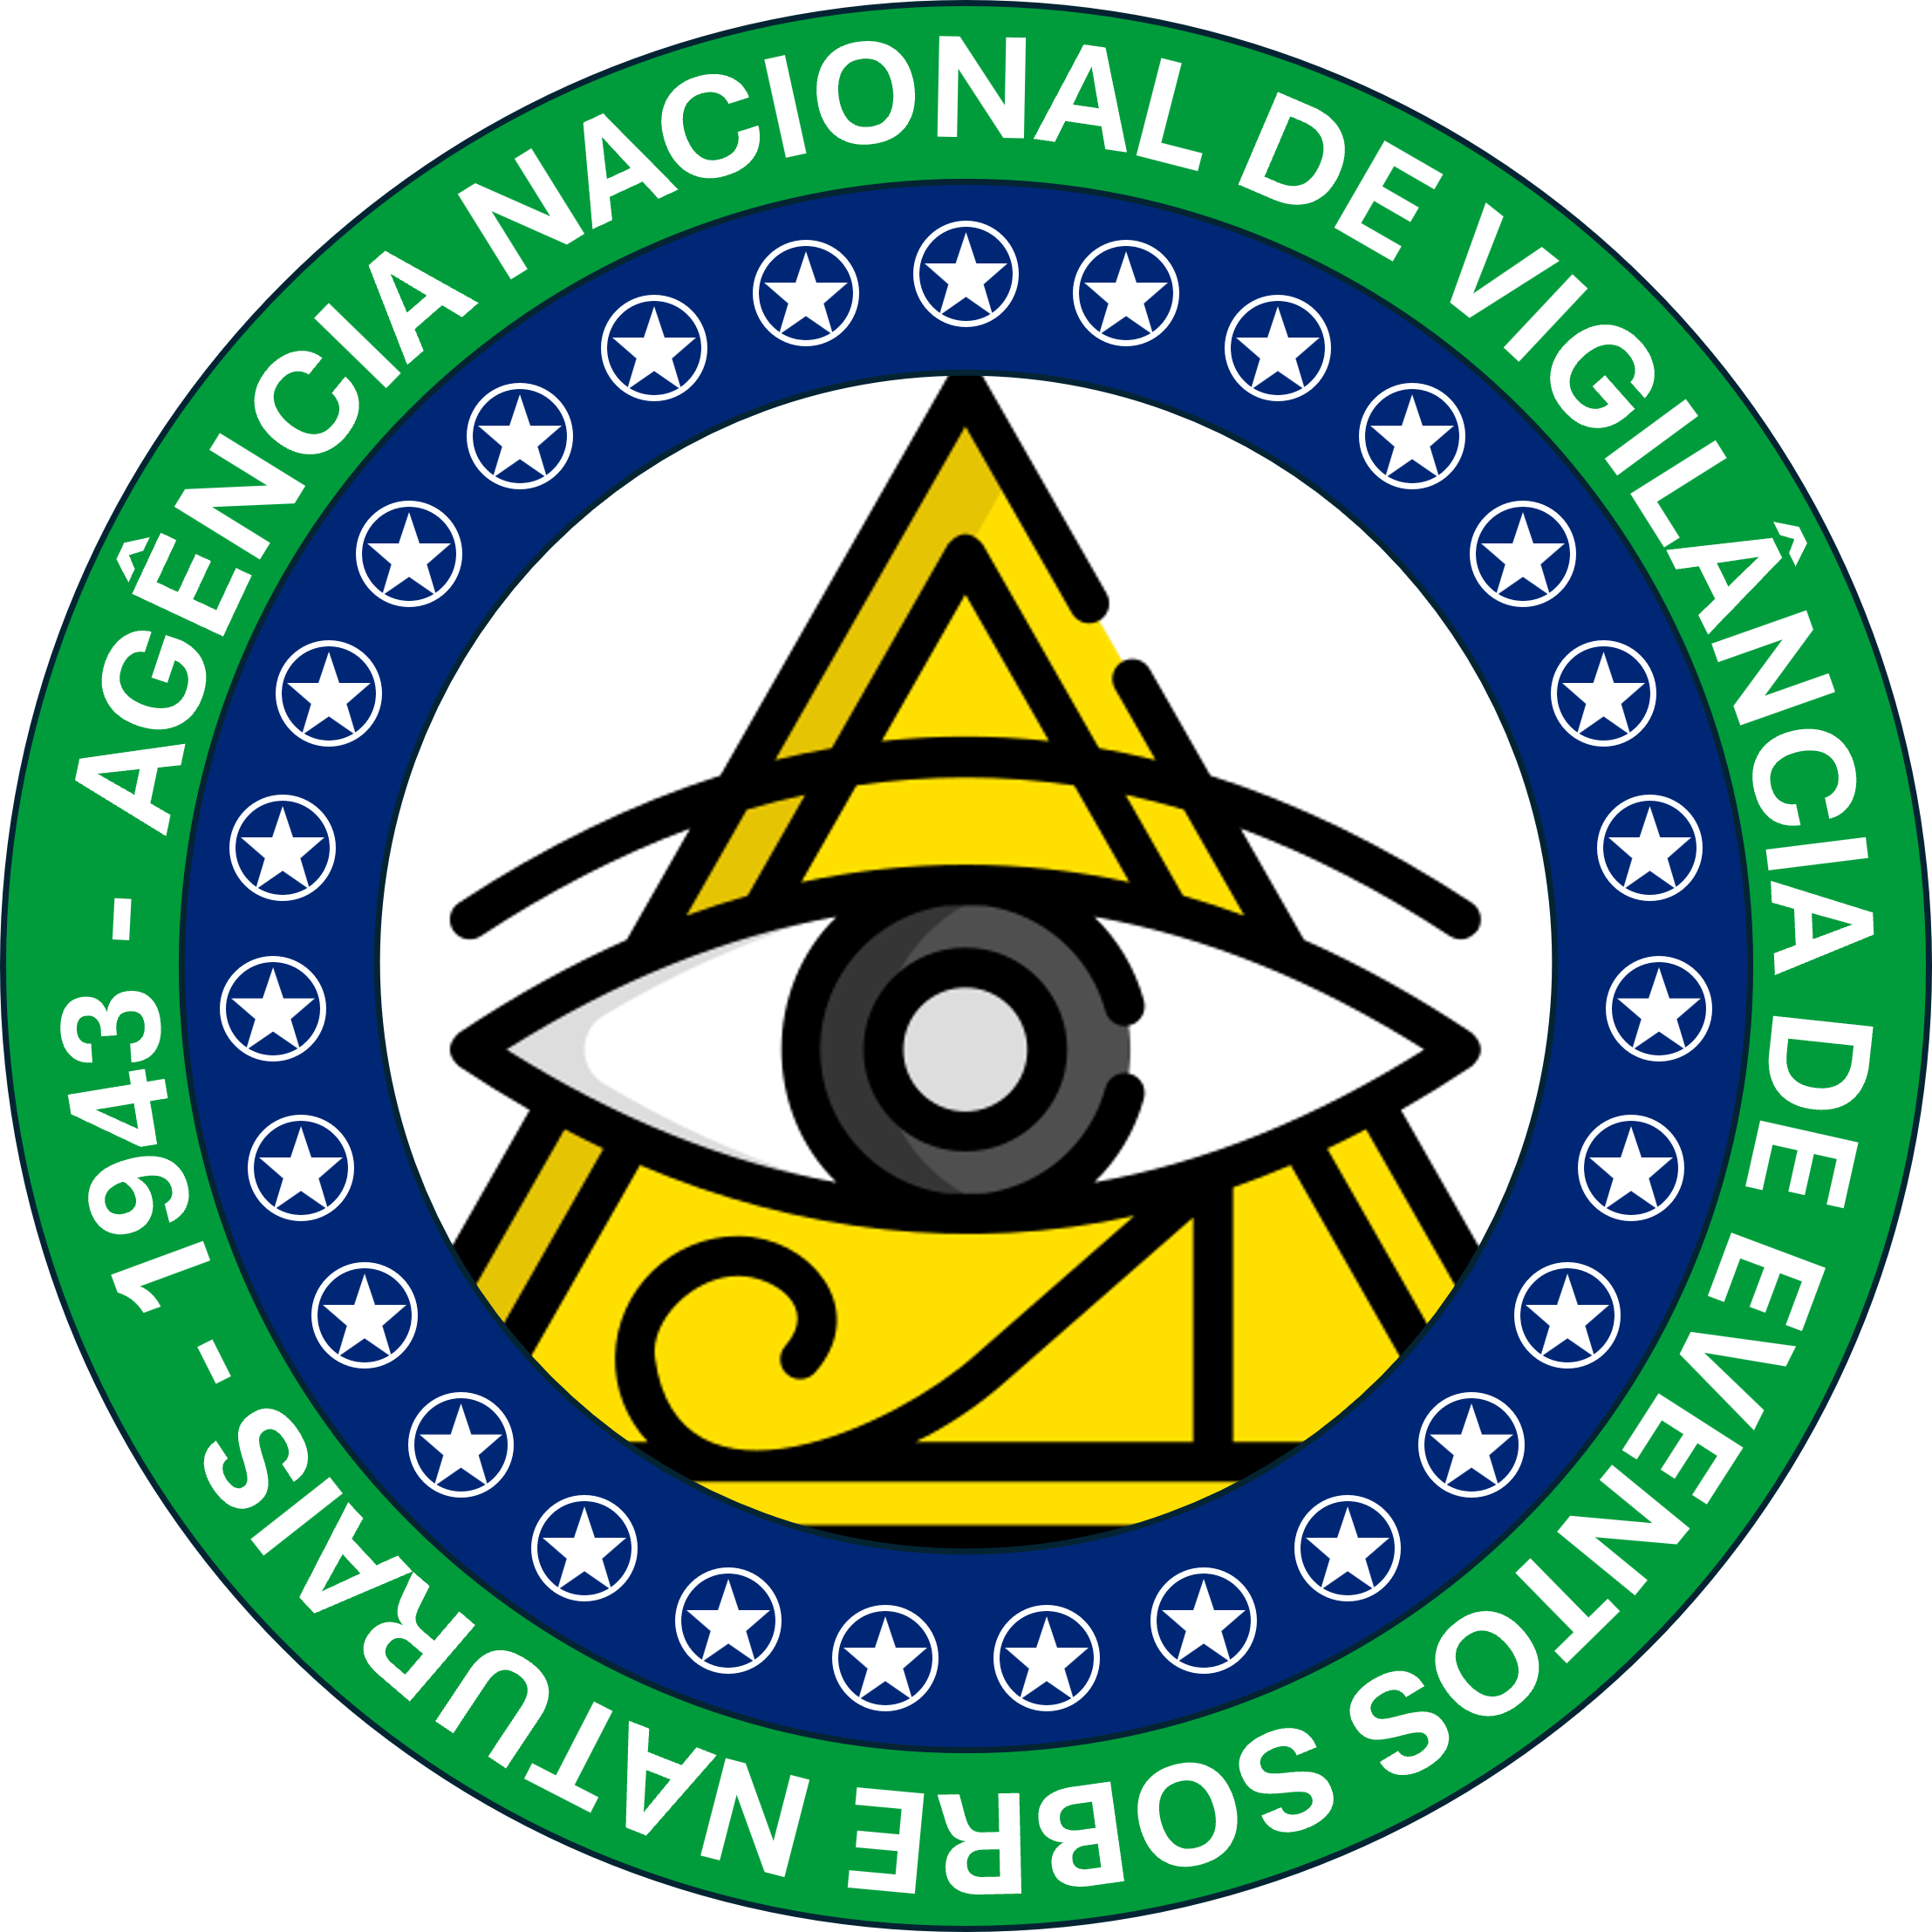
\includegraphics[width=0.5\linewidth]{imagens/ANVESN_LOGO.png}
    \caption{Exemplo de Configuração de Equipamentos em uma Missão de Exorcismo}
    \label{fig:example-setup}
\end{figure}

\end{document}

% (continuação do manual como no texto anterior)
